\documentclass[runningheads]{llncs}

\usepackage{amsmath}
\usepackage{booktabs}
\usepackage{graphicx}
\usepackage{float}
\usepackage{morefloats}
\usepackage[hidelinks]{hyperref}

\renewcommand{\topfraction}{.85}
\renewcommand{\bottomfraction}{.7}
\renewcommand{\textfraction}{.15}
\renewcommand{\floatpagefraction}{.66}
\setcounter{topnumber}{3}
\setcounter{bottomnumber}{2}
\setcounter{totalnumber}{5}

\title{Text Flappy Bird: Monte Carlo vs. Sarsa}
\titlerunning{Text Flappy Bird}

\author{El Jattari Wassim}
\authorrunning{El Jattari Wassim}
\institute{Centralesupélec, Paris, France\\
\email{wassim.eljattari@student-cs.fr}}

\begin{document}
\maketitle

\begin{abstract}
The goal of this work is to implement agents to solve Text Flappy Bird in two settings (without screen and with screen) and compare the performance of different methods. I first train tabular Monte Carlo and SARSA on compact no-screen observations, then test Monte Carlo on raw screen observations. Because raw screen states are too numerous for direct tabular learning, I encode screens into discrete latent vectors and train Monte Carlo on encoded states. This final approach clearly improves over the raw-screen baseline while keeping a tabular control loop.
\keywords{Reinforcement learning \and Flappy Bird}
\end{abstract}

\section{Objective and Environment}
The goal of this work is to implement and compare agents for Text Flappy Bird in no-screen and screen settings. The screen is a matrix containing 3 values (0,1,2). The position of the bird and the pipes are thus integer, so is the distance. I use the two environments available in the gym. \textbf{TextFlappyBird-v0} (no-screen): the state gives the distance between the bird and the center of the next pipe gap. \textbf{TextFlappyBird-screen-v0} (screen): the state is the full grid/screen array. During training I add a score cap (1000) to stop very long episodes and keep runs computationally manageable.

\section{No-Screen Implementation}
\subsection{Monte Carlo Agent}
I first implemented an every-visit Monte Carlo control agent with epsilon-greedy exploration. The first implementation already worked well, but took time to train (100k games).

\begin{figure}[H]
	\centering
    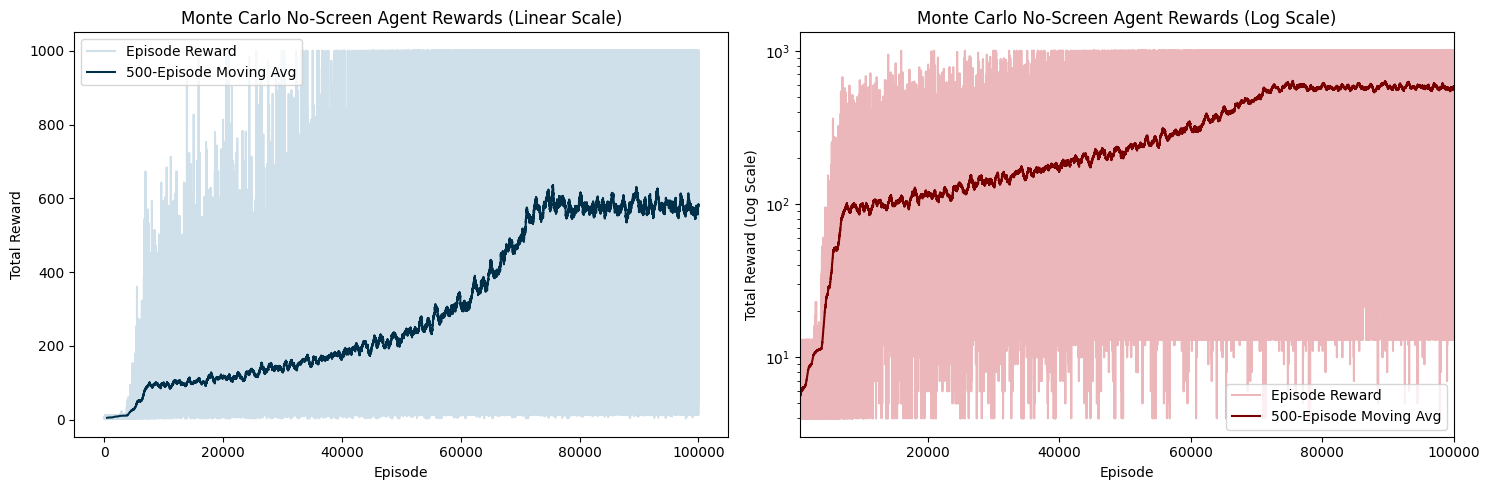
\includegraphics[width=0.9\textwidth]{plots/img_mcns_agent_rewards.png}
	\caption{No-screen Monte Carlo rewards over 100k episodes.}
\end{figure}

\subsection{Hyperparameters and Best Agent}
I explored the main Monte Carlo hyperparameters one-at-a-time: gamma, alpha, epsilon, and epsilon decay. I added an epsilon decay because regardless of the set of parameters I chose, it would always converge toward a reward of 600. This was weird given that I set the maximum to be 1000. In the end I was never able to find out why the reward plateau at 600 since when I run the agent on games, they achieve a max score over 1000 consecutive games.

Their roles and observed influence are:
\begin{itemize}
	\item Gamma controls long-term vs short-term returns. In my runs, this strongly affected final stability of the plateau.
	\item Alpha controls update magnitude. It mostly affected learning smoothness, and also affected the stability of the plateau.
	\item Epsilon controls exploration rate. Too low led to weak exploration; too high slowed exploitation. The lower the epsilon, the better the agent was. But this is mostly because exploration causes failure.
	\item Epsilon decay was critical. A progressive reduction of exploration gave the best compromise between early discovery and late stabilization.
\end{itemize}

With tuned values, I obtained a stronger, faster (40k games) and more stable Monte Carlo run:

\begin{figure}[!ht]
	\centering
	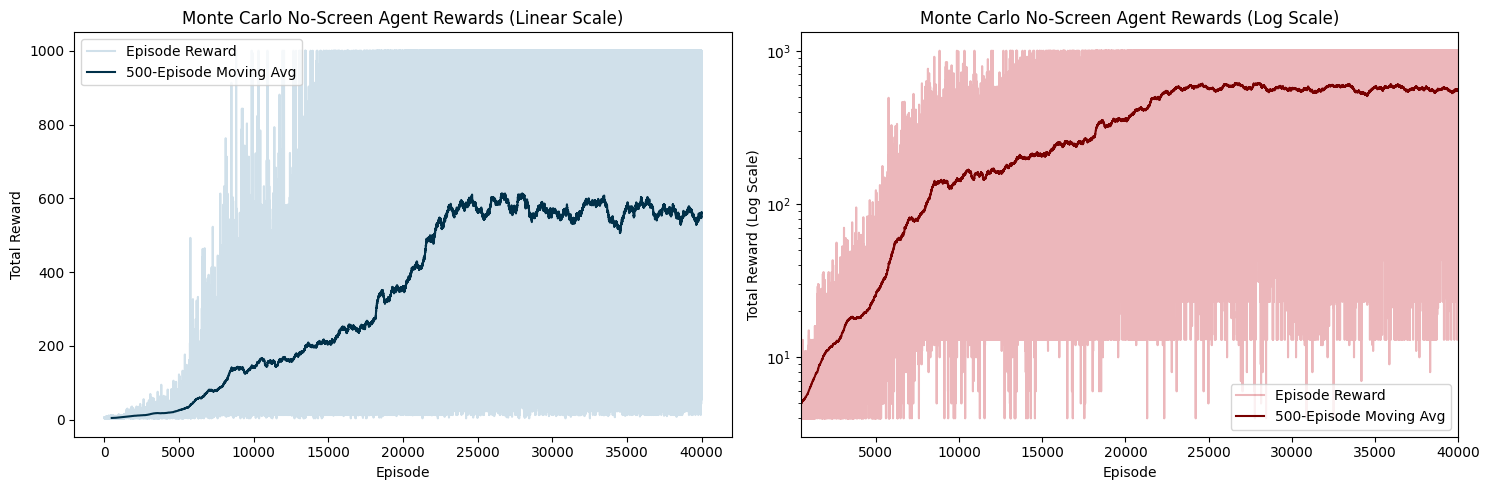
\includegraphics[width=0.9\textwidth]{plots/img_mcns_best_agent_rewards.png}
	\caption{Best no-screen Monte Carlo training curve.}
\end{figure}

\begin{figure}[H]
	\centering
	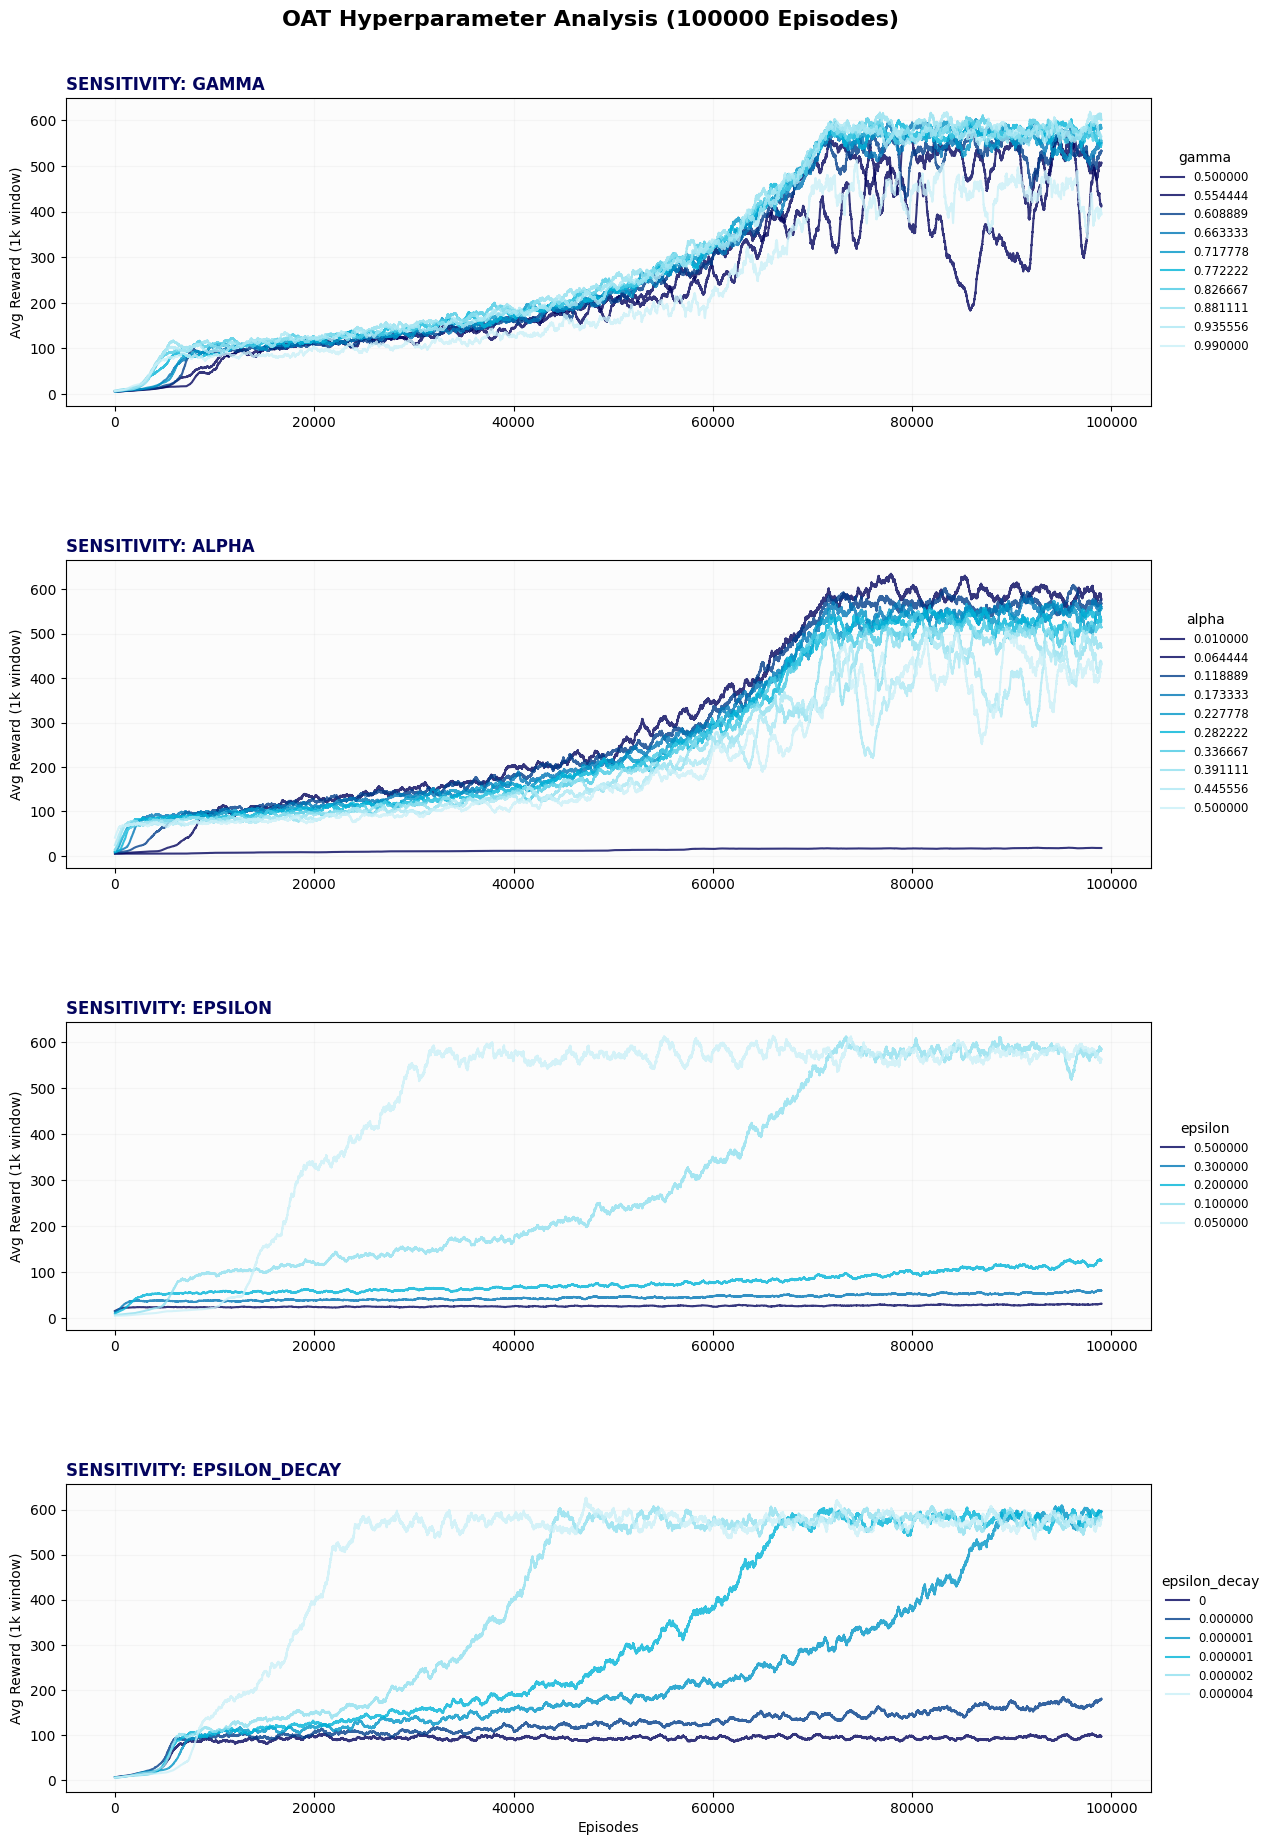
\includegraphics[width=0.87\textwidth]{plots/img_mcns_hyperparamters.png}
	\caption{No-screen Monte Carlo hyperparameter sensitivity study.}
\end{figure}


\subsection{SARSA on No-Screen}
I also implemented SARSA($\lambda$) with eligibility traces.

\begin{figure}[!ht]
	\centering
	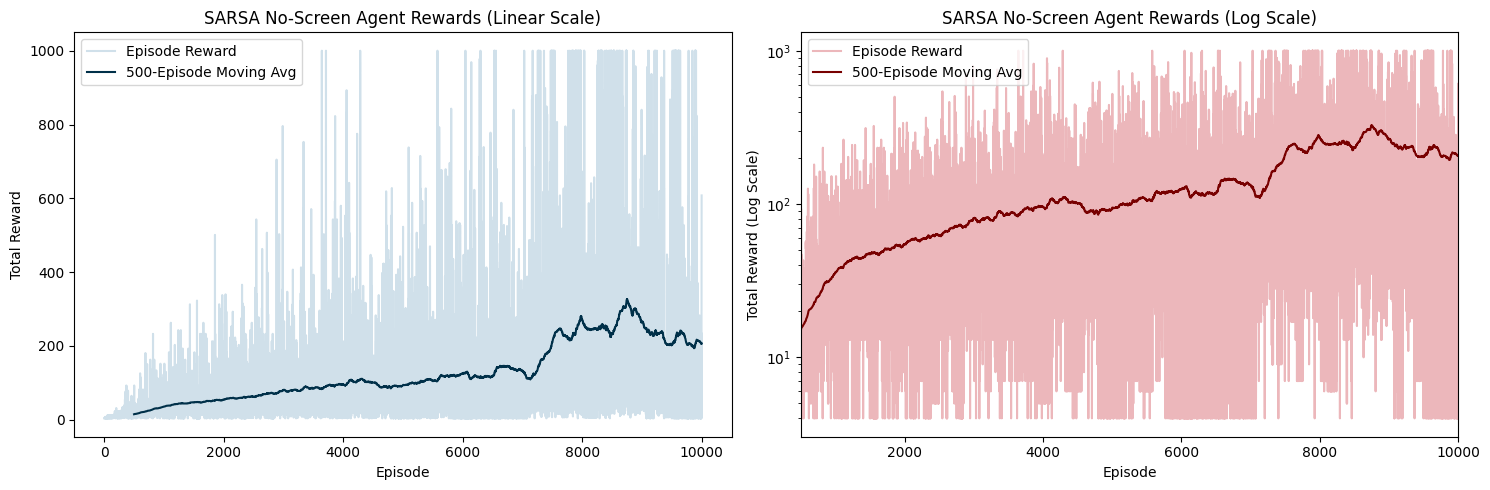
\includegraphics[width=0.9\textwidth]{plots/img_ssns_agent_rewards.png}
	\caption{No-screen SARSA rewards.}
\end{figure}

In practice, SARSA converges in fewer episodes, but it is much slower in wall-clock time, likely because it updates online at each step. I did not run a SARSA hyperparameter sweep for this reason: the Monte Carlo sweep already took about 5 hours, and one SARSA training run was roughly 10 times slower.

\subsection{Performance on other environment}

My implementation of the agent did not perform well when I changed the parameters of the game. The Monte Carlo agent for a game of setting (height=20, width=30, pipe gap=4) when playing 1000 games achieved a mean score of 116 (median 69). This is still decent, but the decrease in performace was to be expected. Especially if the agent is given states that it has never seen.

\section{Screen Flappy Bird}
\subsection{First Attempt: Raw-Screen Monte Carlo}
I first tried using the same tabular Monte Carlo idea directly on raw screen observations (flattened screen as key). Results were weak and did not show satisfactory convergence.

\begin{figure}[!ht]
	\centering
	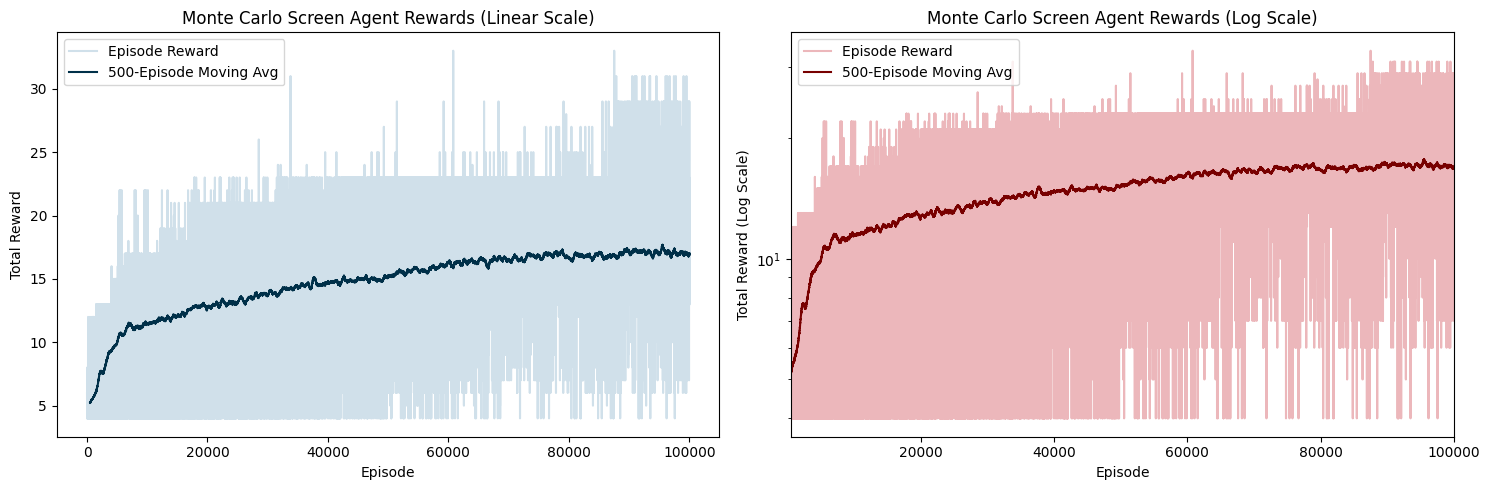
\includegraphics[width=0.9\textwidth]{plots/img_mcs_agent_rewards.png}
	\caption{Raw-screen Monte Carlo baseline.}
\end{figure}

The main reason is likely the huge number of possible states when the full screen is used directly.

\subsection{Encoding the Screen into a Vector}
To reduce the state-space size, I trained autoencoders to encode each screen into a compact latent vector, then discretized the latent values (floored) so they can be used as tabular state identifiers.

I evaluated three model families and multiple settings for latent dimension, hidden size, and latent scale. The loss is from the reconstruction from the floored value.

\begin{figure}[H]
	\centering
	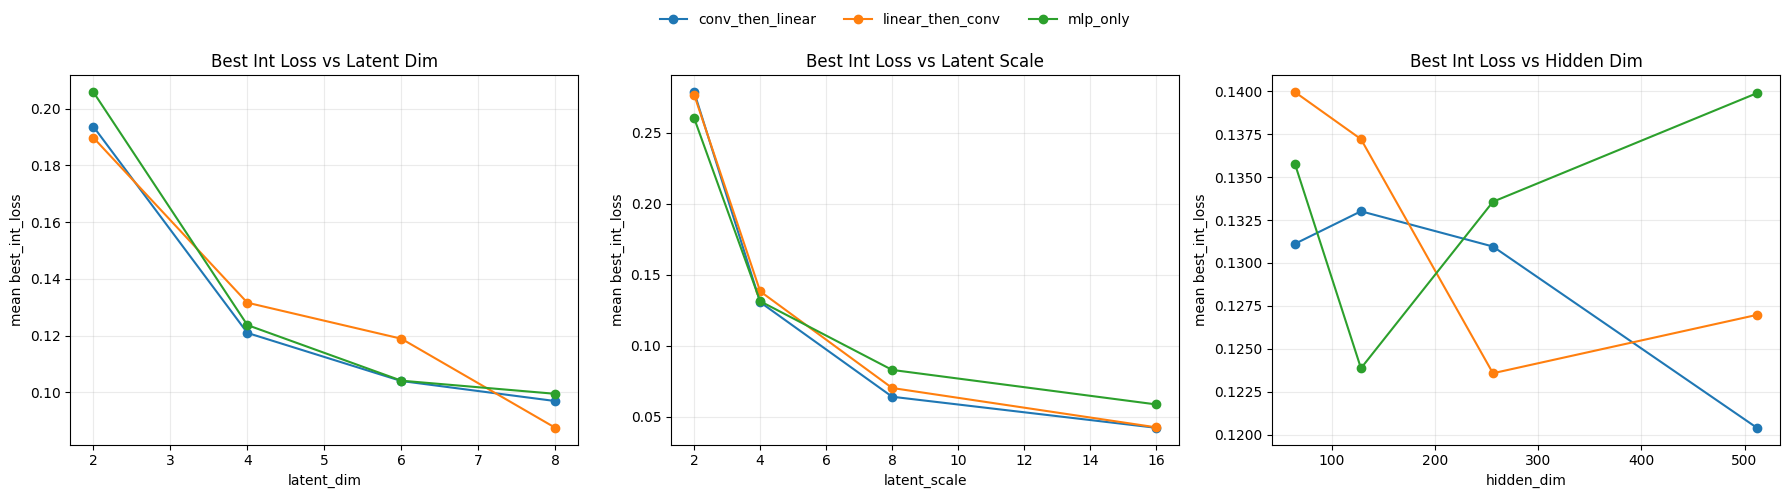
\includegraphics[width=0.99\textwidth]{plots/img_ae_hyperparameters_full.png}
	\caption{Global autoencoder sweep trends.}
\end{figure}

\begin{figure}[H]
	\centering
	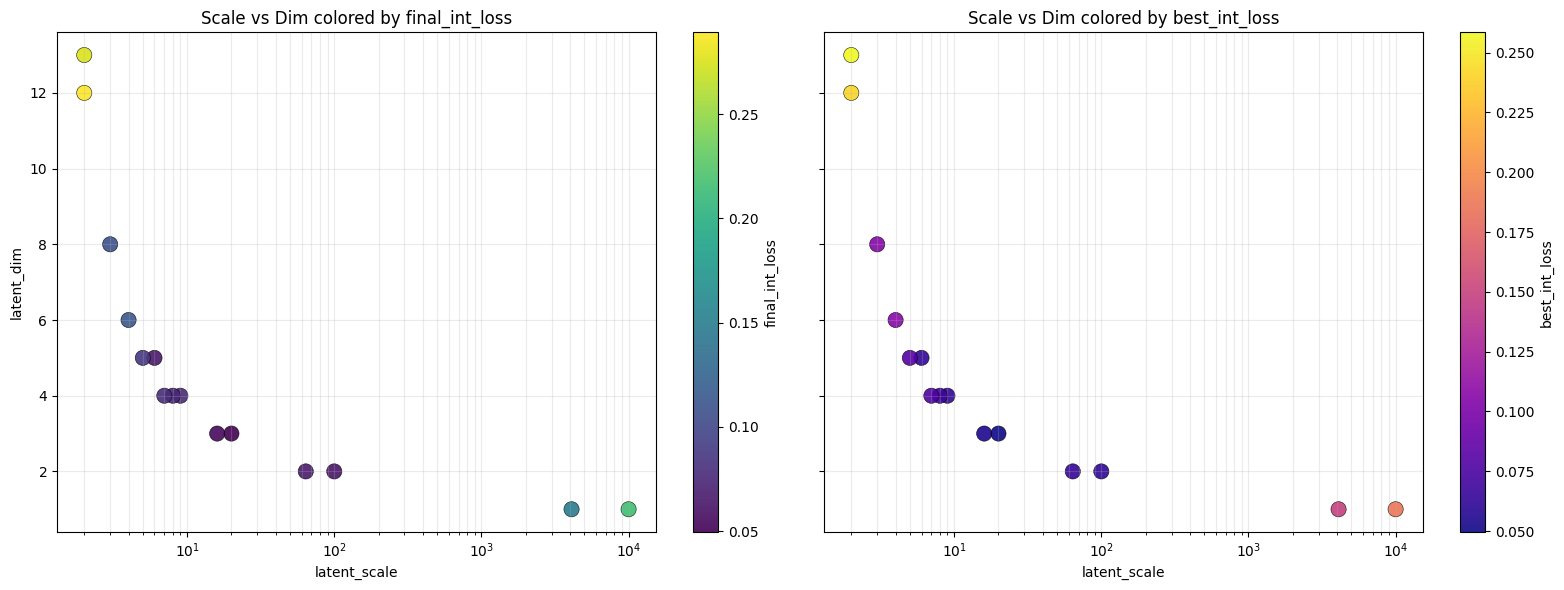
\includegraphics[width=0.9\textwidth]{plots/img_ae_hyperparameters_states_scatter.png}
	\caption{Latent scale vs. latent dimension trade-off.}
\end{figure}

This gave intersting but predictable results. The most important factor for the quality of the encoding is the number of states. In the end I chose $20^3=8000$ as the parameters. To qualitatively validate the encoding pipeline, I also inspected reconstruction dynamics (a GIF is available on the Github Repository).

\section{Monte Carlo on Encoded Screen States}
After encoding, I trained a Monte Carlo agent that uses the discretized latent tuple as the tabular state.

\begin{figure}[!ht]
	\centering
	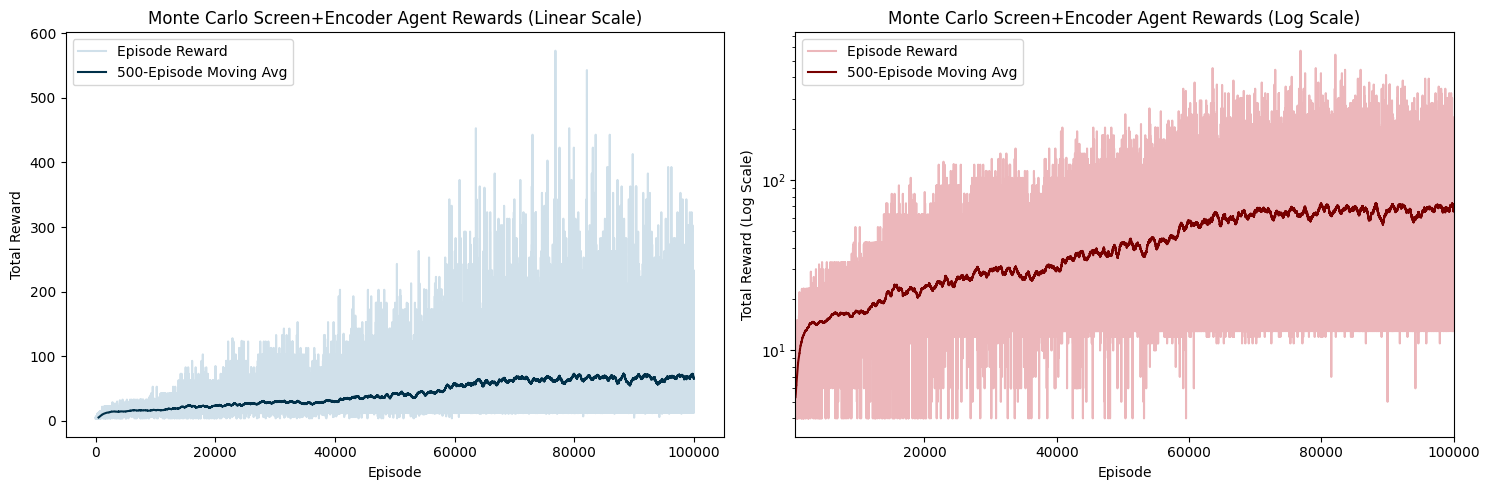
\includegraphics[width=0.9\textwidth]{plots/img_emcs_agent_rewards.png}
	\caption{Monte Carlo training with encoded screen states.}
\end{figure}

Compared with the raw-screen baseline, this encoded version performs substantially better, which supports the idea that representation compression is essential before tabular learning on high-dimensional observations.

\section{Discussion}
My incremental pipeline demonstrates that while tabular methods excel on compact, geometrically informative states, they fail on raw screens due to state-space explosion. I observed a notable trade-off in training dynamics: SARSA converges in fewer episodes through online updates, yet Monte Carlo often proves faster in wall-clock time by processing full trajectories. Ultimately, I find that encoding screens into discrete latent vectors restores tractability, providing a bridge between high-dimensional observations and efficient tabular control. This representation offers the most robust compromise between richness and performance in my study.

\end{document}
